\documentclass[10pt,a4paper]{article}
	\usepackage[french]{babel}
	\usepackage[utf8]{inputenc}
	\usepackage[T1]{fontenc}

	\usepackage{amsmath}
	\usepackage{amsfonts}
	\usepackage{amssymb}
	
	\usepackage{calc}
	\usepackage{subcaption}
	\usepackage{graphicx}

	\usepackage{multicol}
		\setlength{\columnsep}{1cm}

	\usepackage{array}
		\newcolumntype{G}[1]{>{\raggedleft\arraybackslash}m{#1}}
		\newcolumntype{D}[1]{>{\raggedright\arraybackslash}m{#1}}
	\usepackage[squaren,Gray]{SIunits}

	\usepackage{xlop}
	\AtEndDocument{\label{lastpage}}
	
	\usepackage{geometry}
		\geometry{hmargin=2.5cm,vmargin=2.5cm}
	
		\usepackage{eso-pic}
		\newcommand{\HRule}{\rule{\linewidth}{0.5mm}}
		\newcommand{\blap}[1]{\vbox to 0pt{#1\vss}}
		\newcommand\AtUpperLeftCorner[3]{%
		 	\put(\LenToUnit{#1},\LenToUnit{\dimexpr\paperheight-#2}){\blap{#3}}%
		}
		\newcommand\AtUpperRightCorner[3]{%
		  	\put(\LenToUnit{\dimexpr\paperwidth-#1},\LenToUnit{\dimexpr\paperheight-#2}){\blap{\llap{#3}}}%
		}

	\usepackage{fancyhdr}
		\pagestyle{fancy}
		\fancyhfoffset{10pt}
		\lhead{\ecole}
		\chead{\matiere}
		\rhead{\Cusrus}
		\lfoot{\prof}	
		\cfoot{\me}
		\rfoot{\thepage/\pageref{lastpage}}
		\renewcommand{\headrulewidth}{0.4pt}
		\renewcommand{\footrulewidth}{0.4pt}
	 
	\usepackage{color}
		\definecolor{pblue}{rgb}{0.13,0.13,1}
		\definecolor{pgreen}{rgb}{0,0.5,0}
		\definecolor{pred}{rgb}{0.9,0,0}
		\definecolor{pgrey}{rgb}{0.46,0.45,0.48}
	
		\usepackage{xcolor}
		\definecolor{codegreen}{rgb}{0,0.6,0}
		\definecolor{codegray}{rgb}{0.5,0.5,0.5}
		\definecolor{codepurple}{rgb}{0.58,0,0.82}
		\definecolor{backcolour}{rgb}{0.95,0.95,0.92}
	
	\usepackage{listings}
		\lstdefinestyle{mystyle}{  
			    commentstyle=\color{codegreen},
			    keywordstyle=\color{magenta},
			    numberstyle=\tiny\color{codegray},
			    stringstyle=\color{codepurple},
			    basicstyle=\ttfamily\footnotesize,
			    breakatwhitespace=false,         
			    breaklines=true,                 
			    captionpos=b,                    
			    keepspaces=true,                 
			    numbers=left,                    
			    numbersep=5pt,                  
			    showspaces=false,                
			    showstringspaces=false,
			    showtabs=false,                  
			    tabsize=2
		}
		\lstset{style=mystyle}

		\setcounter{tocdepth}{3}

	\usepackage{hyperref}                 
		\hypersetup{
			hyperfigures = true,
			colorlinks = true,
			linkcolor=pblue
			}

%%%%%%%%%%%%%%%%%%%%%%%%%%%%%%%%%%%%%%%%%%%%%%%%%%%%%%%%%%%%%%%%%%%%%%%%%%%%%%%%%%%%%%%%%%%%%%%%
%
% 								Info Perso
%
%%%%%%%%%%%%%%%%%%%%%%%%%%%%%%%%%%%%%%%%%%%%%%%%%%%%%%%%%%%%%%%%%%%%%%%%%%%%%%%%%%%%%%%%%%%%%%%%

% Nom de l'élève			- \me
	\newcommand{\me}{Mathurin \textsc{Cartron}}
% Nom du reférent matière 	- \prof
	\newcommand{\prof}{Maxime \textsc{Maria}} 
% Matière 					- \matiere
	\newcommand{\matiere}{Moteur 3D}
% Cursusse 					- \Cusrus
	\newcommand{\Cusrus}{Master ISICG/CRYPTIS}
% Année dans ce Cursus 		- \Prog			
	\newcommand{\Prog}{Semestre 1}
% Numéros INE 				- \ine
	\newcommand{\ine}{}
% Nom de l'école 			- \ecole
	\newcommand{\ecole}{Université de limoges}
% Titre du document 		- \titre
	\newcommand{\titre}{Projet d'\matiere}
% Sous titre du document 	- \soustitre
	\newcommand{\soustitre}{Compte Rendu}

\author{\me}
\title{\titre}
\date{\today}
\makeatletter

\begin{document}

%%%%%%%%%%%%%%%%%%%%%%%%%%%%%%%%%%%%%%%%%%%%%%%%%%%%%%%%%%%%%%%%%%%%%%%%%%%%%%%%%%%%%%%%%%%%%%%%
%
% 								   Page de garde
%
%%%%%%%%%%%%%%%%%%%%%%%%%%%%%%%%%%%%%%%%%%%%%%%%%%%%%%%%%%%%%%%%%%%%%%%%%%%%%%%%%%%%%%%%%%%%%%%%

	\begin{titlepage}
		\enlargethispage{2cm}
		\begin{center}
			\makebox[\textwidth]{
\includegraphics[width=0.3\paperwidth]{logo.jpg}}\\
			\vspace*{1cm}
			\HRule\\
				\vspace*{.5cm}
				\textsc{\LARGE{\titre}}\\
				\vspace*{.7cm}
				\Large{\soustitre}\\
				\vspace*{.2cm}
			\HRule
			\vspace*{.7cm}
			\begin{tabular}{D{7cm} G{7cm}}
				Élèves :  	&  Professeur : \\
				\me 		&  \prof  \\
			\end{tabular}
		\end{center}
		\vspace*{.7cm}
		\begin{multicols}{2}
			\tableofcontents
			\listoftables
			\listoffigures
			% \lstlistoflistings
		\end{multicols}
		% \centering{\Cusrus -- \Prog \\}
		\vspace*{4cm}
	\end{titlepage}

\ClearShipoutPicture

%%%%%%%%%%%%%%%%%%%%%%%%%%%%%%%%%%%%%%%%%%%%%%%%%%%%%%%%%%%%%%%%%%%%%%%%%%%%%%%%%%%%%%%%%%%%%%%%
%
% 								   Content
%
%%%%%%%%%%%%%%%%%%%%%%%%%%%%%%%%%%%%%%%%%%%%%%%%%%%%%%%%%%%%%%%%%%%%%%%%%%%%%%%%%%%%%%%%%%%%%%%%

\section{Introduction}
	Le but de ce projet est de mettre en œuvre les différentes méthodes vues en cours et en TP, au travers d'une application de visualisation interactive de scènes 3D. L'objectif est d'implémenter des méthodes de rendu temps-réel pour réaliser des effets plus ou moins complexes. Parmi ces effets, on peut citer le light culling, le forward+, le calcul des ombres portées (shadow mapping, shadow volume), l'SSAO, l'FXAA et le bloom. Chacun de ces effets présente des défis spécifiques qui seront abordés dans le cadre de ce projet.

	\paragraph{Une longue absence} % (fold)
		En raison d'une longue absence dont vous connaissez la raison, j'ai pris un lourd retard dans mon travail. Par conséquent, je me contenterai de rendre le travail des TPs malgré les efforts que j'ai pu fournir. Bien que cela ne couvre pas l'ensemble de ce qui était prévu pour ce projet, je suis conscient de l'importance de rendre quelque chose de complet et de bonne qualité. Je ferai de mon mieux pour atteindre cet objectif en privilégiant une bonne compréhension de notion qu'un projet entier mais baclé.
	% paragraph Une longue absence (end)

	\paragraph{Guacamole}
		Malheureusement, j'ai également été confronté à un autre obstacle qui a encore aggravé mon retard : la panne de l'outil "guacamole". Cette panne m'a empêché de travailler pendant les vacances et a considérablement affecté ma progression. Malgré tout, j'ai fait de mon mieux pour rattraper mon retard à la rentrer, même si je ne parviens pas à couvrir tous les aspects prévus pour ce projet.
	% paragraph Guacamole (end)

	\paragraph{De l'aide de mes camarades}
		Heureusement, mes camarades m'ont apporté leur soutien et m'ont aidé à surmonter ces difficultés. Grâce à leur assistance, j'ai pu avancer dans mon travail et commencer à mettre en œuvre les différentes méthodes vues en cours et en TP. Cependant, je dois admettre que, malgré ma volonté de livrer un travail original et indépendant, il y a probablement plus de similarité entre le travail de mes camarades et le mien qu'il n'y en aurait eu sans leur intervention. En effet, ils ont dû déboguer mon code en se servant du leur, ce qui a inévitablement laissé des traces dans mon travail final. Je tiens à préciser que, malgré ces circonstances difficiles, j'ai fait de mon mieux pour assurer l'originalité de mon travail et éviter toute forme de plagiat. Si, malgré mes efforts, il y a des parties de mon travail qui présentent une forte similarité avec celui de mes camarades, je m'engage à le signaler explicitement dans les fichiers code et à préciser les contributions de chacun.
	% paragraph De l'aide de mes camarades (end)
	
\section{Contenu}
	\subsection{Architecture des TP}
		Au début du TP1, nous avons recu un projet qui allait évoluer jusqu'à la fin (TP6). L'objectif était de ne disposer que d'un seul projet Visual Studio, en utilisant un système de lab\_works pour gérer les différentes étapes du projet global.

		\paragraph{}Le lab\_works était organisé de manière à séparer les différents éléments du projet en plusieurs répertoires, chacun ayant un rôle précis :

		\begin{itemize}
			\item Le répertoire "src" contenait le code source du projet, organisé en plusieurs sous-répertoires selon leur fonction (par exemple, "core", "graphics", "input", etc.).
			\item Le répertoire "lib" contenait les bibliothèques externes utilisées par le projet (par exemple, "glew", "glfw", etc.).
			\item Le répertoire "data" contenait les données utilisées par le projet (par exemple, les modèles 3D, les textures, etc.).
		\end{itemize}

		\paragraph{}En utilisant cette architecture, nous avons pu travailler de manière organisée et efficace sur chaque TP, en ajoutant progressivement de nouvelles fonctionnalités au projet.

	\subsection{Le lab\_works\_manager} % (fold)
		En outre, le dossier lab\_works était divisé en sous-dossiers, un pour chaque TP. Ainsi, chaque TP disposait de son propre lab\_works, qui contenait tous les fichiers nécessaires pour compiler et exécuter le projet (shaders et le code du workspace).

		\paragraph{}Pour faciliter la navigation entre les différents lab\_works, nous avons mis en place un lab\_works\_manager. Ce dernier était accessible depuis le menu principal de l'application et permettait de passer d'un lab\_works à l'autre sans avoir à recompiler le code. Cette fonctionnalité a été particulièrement aprécier pour pouvoir comparrer nos différents TP entre eux et entre nous quelque soit l'avancement de chacun.

		\paragraph{Chargement d'un lab\_works} % (fold)
			Pour illustrer comment le lab\_works\_manager fonctionnait, je vais maintenant vous montrer le morceau de code qui permettait de charger un lab\_works. Dans la fonction \texttt{void LabWorkManager::drawMenu()} il suffisait de rajouter et de décliner pour chaque TP le code suivant:

			\lstinputlisting[language=C++ ,firstline=17, lastline=31,caption=Appel d'un lab\_works dans le lab\_works\_manager]{../m3d_isicg-main/src/lab_works/common/lab_work_manager.cpp}
			
		
		% paragraph Chargement d'un lab\_works (end)
	% subsection Le lab\_works manager (end)

	\subsection{Le lab\_works} % (fold)
		La classe LabWork1 est une classe dérivée de BaseLabWork et est utilisée pour implémenter le premier TP. Elle possède les méthodes suivantes :

		\begin{itemize}
			\item[\textbf{init()}] : méthode appelée au lancement de l'application pour initialiser les données de la scène et les données OpenGL.
			\item[\textbf{animate(float)}] : méthode appelée à chaque frame pour mettre à jour les données de la scène.
			\item[\textbf{render()}] : méthode appelée à chaque frame pour dessiner la scène à l'écran.
			\item[\textbf{handleEvents(SDL\_Event)}] : méthode appelée pour gérer les événements envoyés par SDL (par exemple, les entrées clavier ou souris).
			\item[\textbf{displayUI()}] : méthode appelée pour afficher l'interface utilisateur de la scène.
		\end{itemize}
		
		\paragraph{} % (fold)
			La classe LabWork1 possède également plusieurs membres privés qui stockent les données de la scène et les données OpenGL :
		% paragraph (end)
		
		\begin{itemize}
			\item[\textbf{\_triangle}] : un tableau de Vec2f qui contient les coordonnées du triangle à dessiner à l'écran.
			\item[\textbf{\_program}] : un identifiant OpenGL pour le programme de shaders utilisé pour dessiner la scène.
			\item[\textbf{\_vbo}] : un identifiant OpenGL pour le VBO (Vertex Buffer Object) utilisé pour stocker les données du triangle.
			\item[\textbf{\_vao}] : un identifiant OpenGL pour le VAO (Vertex Array Object) utilisé pour stocker les données de configuration de l'attribut de position du triangle.
			\item[\textbf{\_bgColor}] : une Vec4f qui contient la couleur de fond de l'application.
			\item[\textbf{\_shaderFolder}] : une chaîne de caractères qui contient le chemin vers le répertoire où se trouvent les shaders utilisés par cette classe.
		\end{itemize}
		
		\subsubsection{La méthode init()} % (fold)
			La méthode init() s'occupe d'initialiser toutes les données de la scène et de configurer OpenGL. Elle commence par appeler la méthode init() de la classe BaseLabWork, qui s'occupe de configurer SDL et OpenGL. Ensuite, elle charge et compile les shaders nécessaires pour dessiner la scène, crée le VAO et le VBO, et initialise les autres données de la scène.
		% subsubsection La méthode init() (end)

		\subsubsection{La méthode animate(float)} % (fold)
			La méthode animate(float) met à jour les données de la scène en fonction du temps écoulé depuis le dernier frame. Elle peut par exemple animer des objets en fonction de leur vitesse ou de leur accélération.
		% subsubsection La méthode animate(float) (end)

		\subsubsection{La méthode render()} % (fold)
			La méthode render() s'occupe de dessiner la scène à l'écran. Elle commence par nettoyer le framebuffer avec la couleur de fond (\_bgColor) et active le programme de shaders (\_program). Ensuite, elle active le VAO (\_vao) et appelle la fonction OpenGL glDrawArrays() pour dessiner le triangle stocké dans le VBO (\_vbo).
		% subsubsection La méthode render() (end)

		\subsubsection{La méthode handleEvents(SDL\_Event)} % (fold)
			La méthode handleEvents(SDL\_Event) est appelée à chaque frame pour gérer les événements envoyés par SDL. Elle peut par exemple gérer les entrées clavier ou souris pour permettre à l'utilisateur de naviguer dans la scène ou de changer les paramètres de l'application. Ce n'est pas utile dans le premier TP mais pas la suite je déplasserai la caméras avec. 
		% subsubsection La méthode handleEvents(SDL\_Event) (end)

		\subsubsection{La méthode displayUI()} % (fold)
			La méthode displayUI() s'occupe d'afficher l'interface utilisateur de la scène. Elle peut utiliser la bibliothèque de l'interface utilisateur (UI) de votre choix (par exemple, ImGui) pour afficher des éléments tels que des boutons, des sliders, etc. qui permettent à l'utilisateur de contrôler l'application.
		% subsubsection La méthode displayUI() (end)

		\subsection{Présentation des 6 TPs} % (fold)
			Le fonctionnement de lab\_works et lab\_works\_manager restant quasiment le même jusqu'à la fin du TP6 (nous allons bien suur rajouter des chose dedans) Voici une description des 6 sujets de TP que nous avons abordés dans le cadre de ce projet. Ci dessous une image de synthèse de chacun d'entre eux. (\textit{cf} Figure \ref{fig:TPs})

			\begin{figure}[!ht]
				\centering
				\begin{subfigure}[b]{0.32\textwidth}
					\centering
					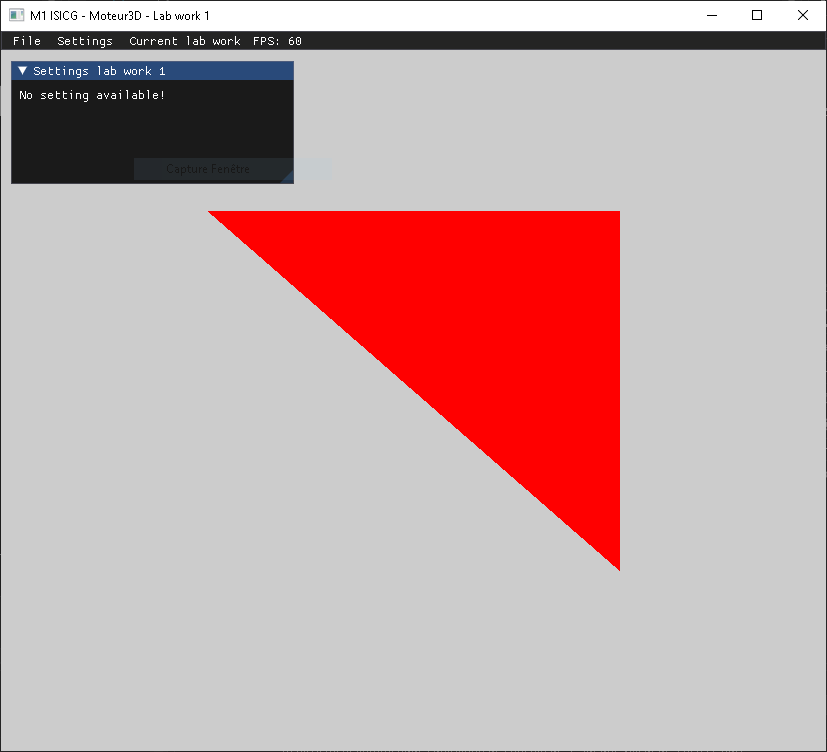
\includegraphics[width=.9\textwidth]{figures/TP1.png}
					\caption{TP1}\label{fig:TP1}
				\end{subfigure}
				\hfill
				\begin{subfigure}[b]{0.32\textwidth}
					\centering
					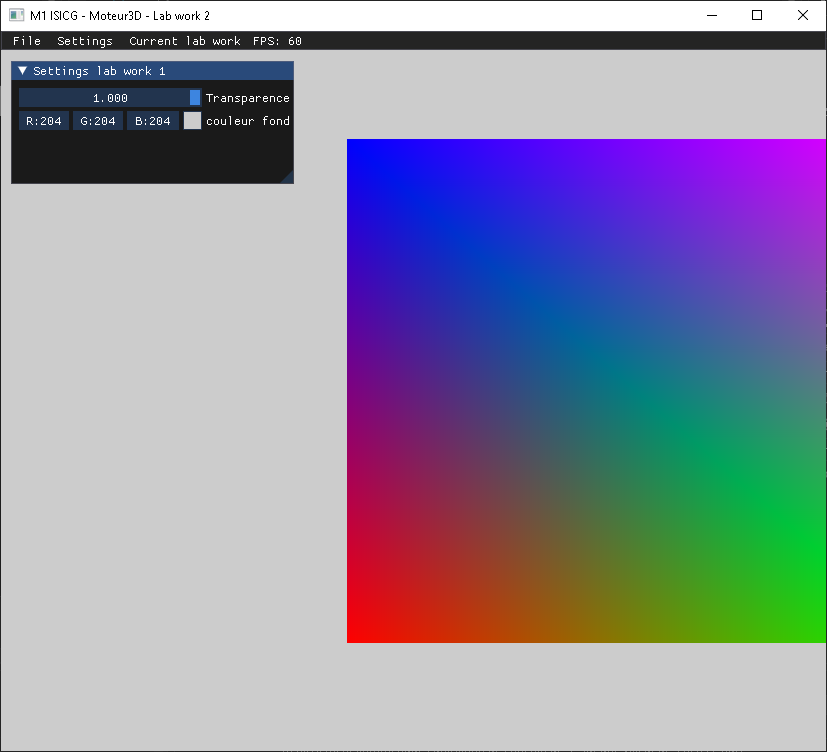
\includegraphics[width=.9\textwidth]{figures/TP2.png}
					\caption{TP2}\label{fig:TP2}
				\end{subfigure}
				\hfill
				\begin{subfigure}[b]{0.32\textwidth}
					\centering
					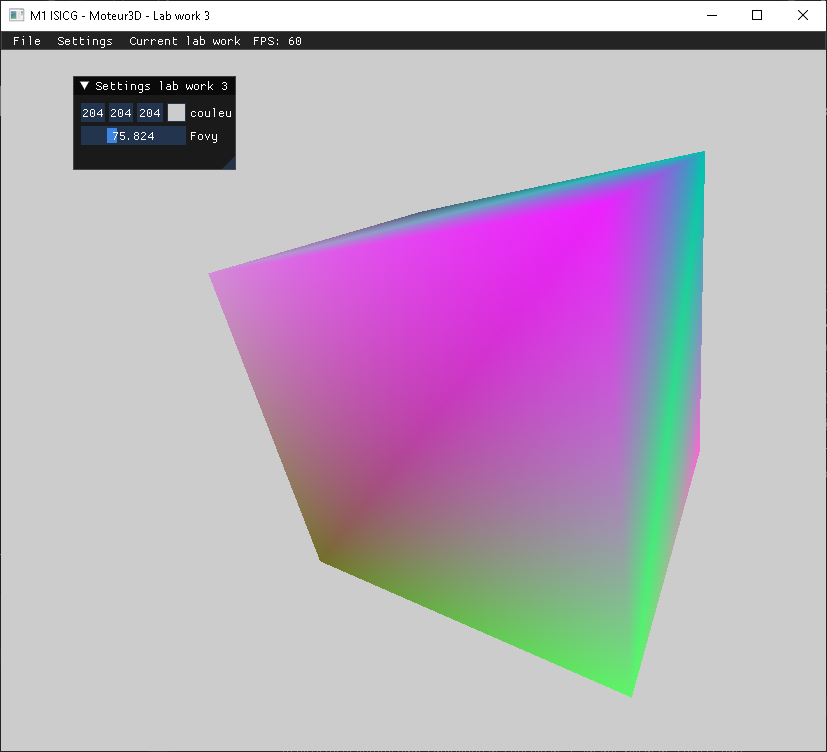
\includegraphics[width=.9\textwidth]{figures/TP3.png}
					\caption{TP3}\label{fig:TP3}
				\end{subfigure}
				\hfill
				\begin{subfigure}[b]{0.32\textwidth}
					\centering
					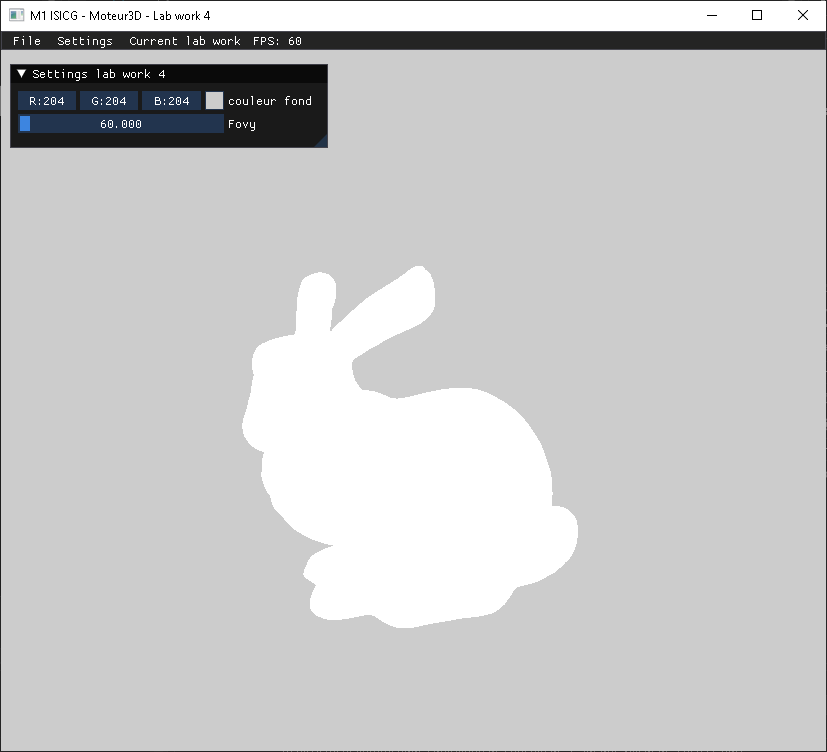
\includegraphics[width=.9\textwidth]{figures/TP4.png}
					\caption{TP4}\label{fig:TP4}
				\end{subfigure}
				\hfill
				\begin{subfigure}[b]{0.32\textwidth}
					\centering
					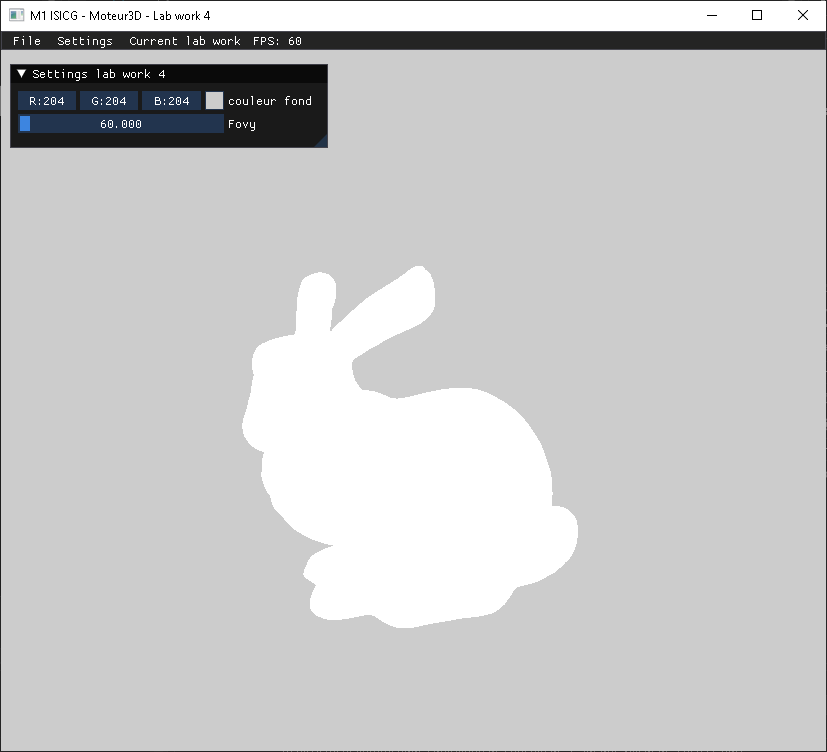
\includegraphics[width=.9\textwidth]{figures/TP5.png}
					\caption{TP5}\label{fig:TP5}
				\end{subfigure}
				\hfill
				\begin{subfigure}[b]{0.32\textwidth}
					\centering
					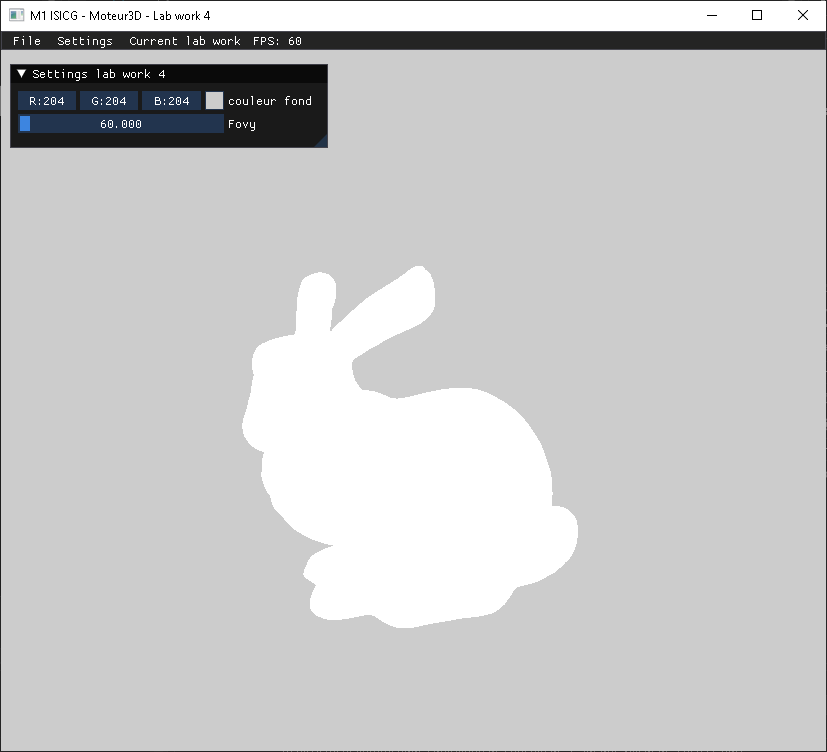
\includegraphics[width=.9\textwidth]{figures/TP6.png}
					\caption{TP6}\label{fig:TP6}
				\end{subfigure}
				\caption{Rendu de touts les TPs}\label{fig:TPs}
			\end{figure}
		
			\subsubsection{TP1}
				L'objectif de ce TP était simplement d'afficher un triangle en 2D sur le plan image. Pour ce faire, nous avons dû apprendre à utiliser les fonctionnalités de base de OpenGL, telles que la création d'un programme de shaders, la gestion de VAO et de VBO, et l'utilisation de glDrawArrays().  (\textit{cf} Figure \ref{fig:TP1})
			% subsubsection TP1 (end)
			
			\subsubsection{TP2}
				Dans le TP2, nous avons affiché un quad en utilisant un VBO de type "Indexed" et en utilisant des shaders de couleur. Nous avons également animé le quad en le faisant se déplacer de gauche à droite et en modifiant son opacité.  (\textit{cf} Figure \ref{fig:TP2})
			% subsubsection TP2 (end)

			\subsubsection{TP3}
				Le TP3 a consisté à afficher un cube multicolore qui tournait sur lui-même en utilisant une caméra freefly. Nous avons appris à créer et à manipuler une matrice de vue pour contrôler la position et l'orientation de la caméra. (\textit{cf} Figure \ref{fig:TP3})
			% subsubsection TP3 (end)

			\subsubsection{TP4}
				Dans le TP4, nous avons chargé un modèle 3D depuis un fichier (le bunny) et avons calculé l'éclairage local de se model. Nous avons aussi vue les éclairages plus avancer comme l'éclairage diffus et l'éclairage spéculaire du model de Phong. (\textit{cf} Figure \ref{fig:TP4})
			% subsubsection TP4 (end)

			\subsubsection{TP5}
				Le TP5 visait à manipuler des textures discrètes pour changer l'apparence de nos objets. Nous avons appris à charger et à appliquer des textures sur nos modèles 3D en utilisant des shaders de texture. (\textit{cf} Figure \ref{fig:TP5})
			% subsubsection TP5 (end)
			
			\subsubsection{TP6}
				Le TP6 a consisté à mettre en place un pipeline de deferred rendering et à appliquer un post-traitement simple sur notre image. Nous avons appris à utiliser les techniques de deferred rendering pour séparer les différentes composantes de notre scène (couleur, position, normale, etc.) et à effectuer un rendu en plusieurs étapes pour obtenir une image finale de meilleure qualité. Nous avons également appris à utiliser les techniques de post-traitement pour améliorer l'apparence de notre image finale (par exemple, en utilisant l'effet de bloom). (\textit{cf} Figure \ref{fig:TP6})
			% subsubsection TP6 (end)

		% subsection Présentation de 6 TP (end)
	
	% subsection Le lab\\_works (end)

\section{Conclusion}

%%%%%%%%%%%%%%%%%%%%%%%%%%%%%%%%%%%%%%%%%%%%%%%%%%%%%%%%%%%%%%%%%%%%%%%%%%%%%%%%%%%%%%%%%%%%%%%%
%
% 								   Exemple
%
%%%%%%%%%%%%%%%%%%%%%%%%%%%%%%%%%%%%%%%%%%%%%%%%%%%%%%%%%%%%%%%%%%%%%%%%%%%%%%%%%%%%%%%%%%%%%%%%

%%%%%%%%%%%%%%%%%%%%% TABLE

% \begin{table}[!ht]
% 	\centering
% 	\begin{tabular}{|*{9}{c|}}
% 		\multicolumn{9}{c}{RGB2HSV}\\								
% 		\hline
% 		block					& 8x8		& 16x16		& 32x32	 	& 	64x64	& 128x128	& 256x256	& 512x512	& 1024x1024 \\
% 		\hline
% 		temps nvproof (us)		& 118,72	& 71,808	& 76,515 	& 	x		& x			& x			& x			& x \\
% 		temps chronoGPU (us)	& 125,76	& 77,856	& 84,416 	& 	x		& x			& x			& x			& x \\
% 		\hline
% 		\multicolumn{9}{c}{HSV2RGB 1D} \\
% 		\hline
% 		block					& 8x1		& 6x1		& 32x1		& 64x1		& 128x1		& 256x1		& 512x1		& 1024x1 \\
% 		\hline
% 		temps nvproof (us)		& 325,28	& 174,85	& 99,328	& 69,494	& 70,206	& 73,355	& 78,725	& 84,589 \\
% 		temps chronoGPU (us)	& 332,256	& 179,952	& 110,624	& 75,36		& 81,312	& 82,672	& 84,512	& 96,288 \\
% 		\hline
% 	\end{tabular}
% 	\caption{Comparatif de temps }\label{tab:temps}
% \end{table}

%%%%%%%%%%%%%%%%%%%%% SUBFIGURE
		
% \begin{figure}[!ht]
% 	\centering
% 	\begin{subfigure}[b]{0.32\textwidth}
% 		\centering
% 		\includegraphics[width=.9\textwidth]{../screens/serie_0_3_20_600_600.png}
% 		\caption{Aléatoire}\label{fig:1}
% 	\end{subfigure}
% 	\hfill
% 	\begin{subfigure}[b]{0.32\textwidth}
% 		\centering
% 		\includegraphics[width=.9\textwidth]{../screens/serie_1_3_20_600_600.png}
% 		\caption{Permutation aléatoire}\label{fig:2}
% 	\end{subfigure}
% 	\hfill
% 	\begin{subfigure}[b]{0.32\textwidth}
% 		\centering
%  		\includegraphics[width=.9\textwidth]{}
% 		\caption{Coupe optimale}\label{fig:3}
% 	\end{subfigure}
% 	\caption{Comparaison des différents algorithmes}\label{fig:rendu}
% \end{figure}


\end{document}